\documentclass[czech,SP]{thesiskiv}

\author{Petr Holický}
\declarationmale

\title{Generování konečného automatu}
\titlepageyear{\today}

\usepackage[nottoc,notlot,notlof]{tocbibind}
\usepackage[pdftex]{graphicx}
\usepackage[pdftex]{hyperref}
\hypersetup{colorlinks=true,
  unicode=true,
  linkcolor=black,
  citecolor=black,
  urlcolor=black,
  bookmarksopen=true}
\usepackage[numbers,sort&compress]{natbib}

%%%%%%%%%%%%%%%%%%%%%%%%%%%%%%%%%%%%%%%%%%%%%%%%%%%%%%%%%%
\begin{document}
%
\maketitle
\tableofcontents

\chapter{Analýza úlohy }
{Tato úloha přináší tři hlavní problémy: čtení ze souboru, generace kódu a implementace samotného konečného automatu. Myslím si, že začít implementací konečného automatu je nejlehčí způsob, protože pokud máme fungující automat tak jen zbývá vymyslet, jak tento kód generovat automaticky.} 
\\
\begin{figure}[!ht]
\centering
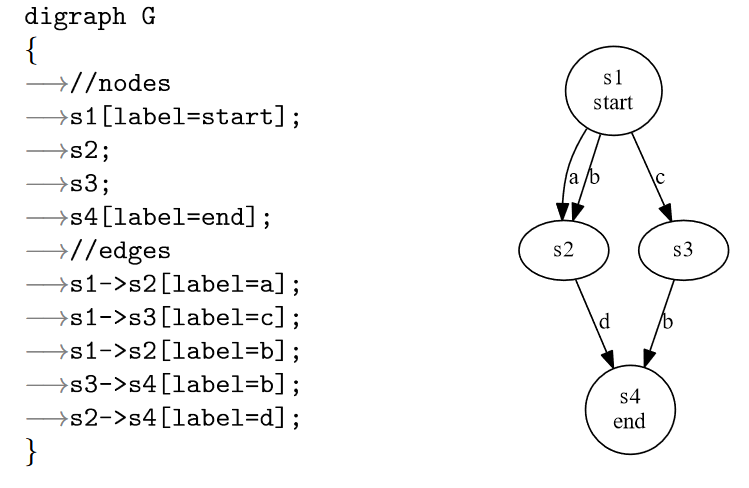
\includegraphics[width=\textwidth]{img1} 
\caption{Ukázka vstupního souboru}
\label{fig:Ukazka}
\end{figure}
\\
{Jako řešení realizace automatu se nabízí tvorba vlasní struktury. Tuto strukturu jsem během chodu programování několikrát změnil a předělal. Hlavní příčinou bylo, že automat se tvořil nejdříve nahráním všech vrcholů, a až poté všemi hranami, viz.(\ref{fig:Ukazka}). Zápasil jsem s problémem přiřazení hran jejich příslušným vrcholům a samotným pohybem mezi vrcholy, které ještě nemají žádné hrany. Tento problém jsem vyřešil rozdělením strukrury na dvě struktury, které na sebe odkazují.  }
\\ \\
{Čtení ze souboru není moc obtížné, celé to stojí na rozhodnutí, po jakých částek budeme soubor načítat. Možnost načítání po znaku jsem vyloučil, protože mi přijde, že by obsahoval příliš mnoho matoucích podmínek. Takže zbývá načítání po vybraných částech, nebo načtení celého řádku a jeho následovné rozebrání. Zvolil jsem možnost načítání celého řádku, jelikož vstupní soubor je napsán vždy stejnou strukturou (viz.(\ref{fig:Ukazka})), tak lze použít stejné podmínky pro více vstupních souborů.}
\\ \\ 
{Se samotným generováním jsem si dlouho nevěděl rady. Jako nejvíce přímočaré řešení mi přpadá, že je zápis do souboru, který se přizpůsobí datům načteným ze vstupního souboru. Zde jsem narazil na problém s objemem zapsaných dat. Vždy zapisovat všechny příslušné funkce mi přišlo zbytečné. Nejdríve jsem uvažoval nad tvorbou univerzálního souboru, který bude obsahovat části, které budou stejné pro všechny vygenerované automaty a tyto části budu postupně číst a následovné zapisovat do výstupního souboru. Ale nakonec jsem zvolil možnost, že si vytvořím vedlejší soubor s funkcemi, které poté budu jednoduše importovat tím, že do výstupního souboru zapíši \texttt{\#include}. }

\chapter{Popis implementace }
{Automat je implementován přes dvě struktury. První struktura pro vrcholy, která obsahuje název vrcholu, jeho label a pole hran, které vychází z tohoto vrcholu. Všechny vrcholy jsou navíc spojené přes spojový seznam. Druhá strukrura pro hrany obsahuje label, název vrcholu ze kterého vychází, ve kterém končí a na odkaz něj. Obě struktury a všechny funkce spojené s konečným automatem jsou obsaženy v souboru \texttt{fsm.h}.} 
\\
\begin{figure}[!ht]
\centering
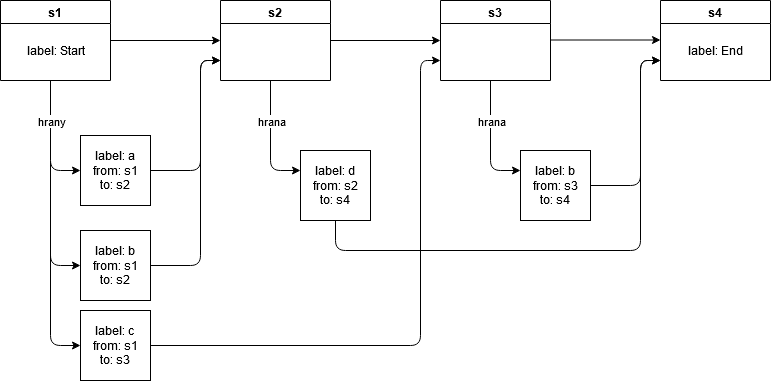
\includegraphics[width=\textwidth]{struct} 
\caption{Ukázka automatu realizovaného použitými strukturami}
\label{fig:Struktura}
\end{figure}
\\
{Funkce jsou rozepsány v souboru \texttt{fsm\_template.c}. První funkce \texttt{add\_node} vytvoří nový vrchol z předaných paramerů, alokuje pole vrcholů a přidá vrchol do spojového seznamu. Druhá funkce \texttt{add\_edge} vytvoří novou hranu z předaných paramerů, přiřadí hranu do pole vrcholu ze kterého vychází a uloží si odkaz na vrchol ve kterém končí. Díky spojovému seznamu vrcholů můžeme vrcholy procházet i bez hran a po načtení všech hran se můžeme hýbat mezi vrcholy přes odkazy uložené v každé hraně. Implementace automatu z obrázku \ref{fig:Ukazka} do struktur je znázorněna na obrázku \ref{fig:Struktura}.} 
\\ \\
{Další funkce \texttt{process} prochází automat podle zadaného řetězce. Vrcholy prochází postupně znak po znaku. V aktuálním vrcholu se projdou všechny jeho hrany a znak se porovná se znakem u každé hrany. Pokud se znaky shodují, přejdeme na další vrchol na který daná hrana odkazuje. Podle pravidel konečného automatu, pokud je zadán znak, který nelze zpracovat nebo řetězec končí na vrcholu který není výstupní, tak se vypíše chybová hláška o nepřijatelném vstupním řetězci. Jinak se vypíše, že řetězec je přijatelný, a vrchol na kterém se skončilo. Poslední funkce \texttt{free\_all} uvolní všechny vrcholy a hrany z paměti.}
\\ \\
{Hlavní soubor \texttt{fsmgen.c} obsahuje pouze dvě funkce. První funkce \texttt{main} nejprve zkontroluje vstupní argumenty a pokusí se otevřít soubor s názvem načteným ze zadaného argumentu. Pokud otevření selže nebo argumenty jsou zadány chybně, program skončí a vypíše chybovou hlášku. Jestliže vstupní argumenty jsou platné a soubor se podařilo otevřít, vytvoří se nový soubor \texttt{fsm.c}, což je výstupní soubor, do kterého se bude zapisovat.} 
\\ \\
{Jako první věc se zapíše \texttt{\#include fsm\_template.c} pro připojení souboru se všemi potřebnými funkcemi pro vytvoření konečného automatu a práci s ním. Dále se zapíše první polovina funkce main, kde se kontrolují vstupní argumenty. Pak se postupně načítají celé řádky ze vstupního souboru. Jednotlivé řádky se rozebírají podle znaků, které uvozují jednotlivé části informací potřebné pro zapsání. Zápis volání funkcí pro tvorbu vrcholů a hran \texttt{add\_node} a \texttt{add\_edge} má dva módy. Pokud se načte řádka obsahující \texttt{//nodes}, tak se zápís přepne do módu 1. V tomto módu se nejdříve zapíše název vrcholu, který je vždy na začátku řádky s odsazením. Pro odebrání bílích znaků se volá druhá funkce \texttt{trim\_space}. Po odstranění bílích znaků se název vrcholu zapíše do parametrů volající funkce. Pokud řádek obsahuje znak \texttt{[} tak to znamená, že obsahuje i label. Label se  téže vyřízne z načtené řádky a zapíše do výstupního souboru. Druhý mód pro zápis hran se spustí po načtení řádky s \texttt{//edges}. Hrany se obdobně jako vrcholy zapisují přes rozebrání načtené řádky. První informace na řádce je vrchol ze kterého hrana vychází, téže obsahující bílé znaky kvůli odsazení. Druhá informace je vrchol ve kterém hrana končí. Poslední informace je label dané hrany. Vstupní soubor je vždy ukončen znakem \texttt{\}}, který vrátí zápis zpět do výchozího módu.} 
\\ \\
{Po načtení a zápisu všech vrcholů a hran se zapíše zbytek funkce \texttt{main}. Ten obsahuje volání funkce \texttt{process} a \texttt{free\_all}. Výspupní soubor \texttt{fsm.c} tedy obsahuje pouze připojení souboru obsahující všechny funkce pro práci s konečnými automaty a funkci \texttt{main}, která vytváří konečný automat a volá funkci \texttt{process} pro zpracování vstupního řetězce načteného z argumentu.}

\chapter{Uživatelská příručka }
{Příkazem \texttt{make} se vytvoří spustitelný soubor \texttt{fsmgen}. Pokud tento soubor spustíme s argumentem, který představuje název vstupního souboru, tak se vytvoří soubor \texttt{fsm.c}. Tento soubor poté musíme ručně přeložit přes gcc překladač. Výsledný spustitelný soubor spustíme s argumentem, který představuje vstupní řetězec pro konečný automat.}

\chapter{Závěr }
{Myslím si, že vhledem k tomu, jak moc jsem byl zprva z jazyka C zmaten, tak nakonec se mi program celkem povedl. Jsem si jist, že některé moje postupy a řešení nejsou úplně dokonalé. Generování kódu zápisem, kde jedním \texttt{fwrite} zapíši dost dlouhý řetězec mi přijde celkem neelegantní, ale ve výsledku to cíl splní. Také pokud samotý obsah vstupního souboru by byl nějak odlišný, tak mnou zvolené řešení by si s tím moc neporadilo. Jinak si myslím, že zbytek je v pořádku a cíl zadání splňuje tak jak má.}


 


\end{document}
